\setcounter{page}{1} \pagenumbering{Alph}

% Add PDF bookmark 
\pdfbookmark[0]{Title}{Title}

%%% LOGO
\thispagestyle{empty}
\begin{flushleft} ~\\ \vspace{-12mm} \hspace{-12mm}  
\includegraphics[width=50mm]{Cover/istnewlogo} 
 
 %%% Instituição
\centering
\LARGE \textbf{UNIVERSIDADE DE LISBOA \\ INSTITUTO SUPERIOR TÉCNICO}
%%% espaço sem gráficos
\vspace{10mm}

%%% Optional Image
%\vspace{10mm}
%~\\ \vspace{50mm} % gráficos
%\\ \begin{center} 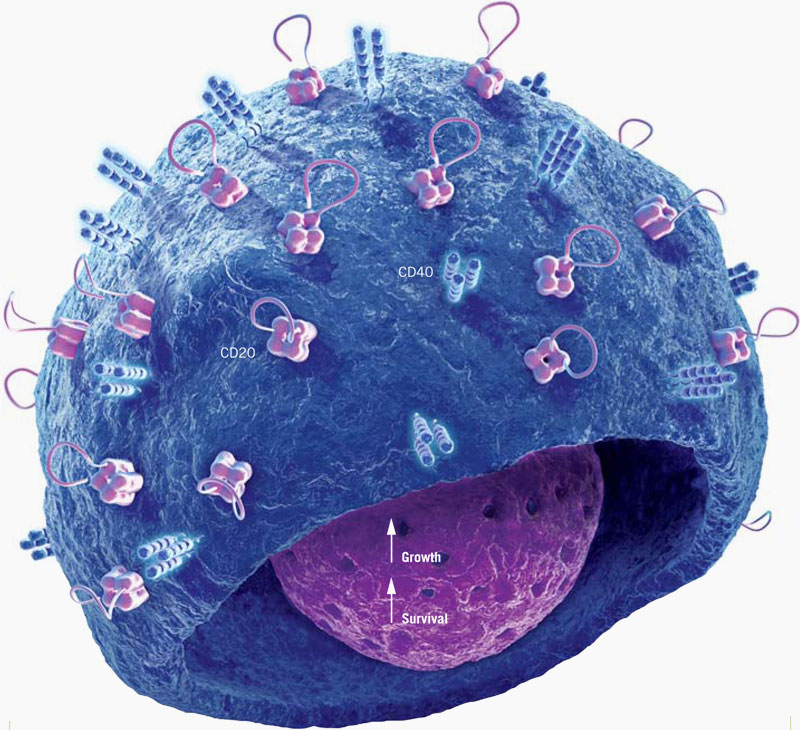
\includegraphics[height=50mm]{Cover/coverimage}  \end{center} % gráficos
 %\vspace{5mm}
 
 %%% Titulo
\centering
\Large \textbf{Título da Tese que descreve o objeto de estudo}
%\\ \vspace{2mm}
%\Large Subtítulo Opcional
\\ \vspace{8mm}
%\\ \vspace{25mm}  % NO SUBTITLE
\Large \textbf{Nome completo} \\
\vspace{8mm}

%Orientadores
\Large
\begin{minipage}{\textwidth}
\begin{tabularx}{\textwidth}{ l @{ } l }
\textbf{Orientador} : & \textbf{Doutor Nome completo}\\
\textbf{Co-Orientador} :  & \textbf{Doutor Nome completo}\\
 %&    ~~~~~~~~~~~~~~~~~~~~~~~~~~ large name\\
\end{tabularx}
\end{minipage}
\\ \vspace{8mm}
\centering
\Large \textbf{Tese aprovada em provas públicas para a obtenção do grau de Doutor em}\\
\Large Engenharia Mecânica\\
\vspace{5mm}
\Large \textbf{Qualificação atribuída pelo Júri: Aprovado}
%\Large \textbf{Qualificação atribuída pelo Júri: Aprovado com Distinção.}
 
\vspace{8mm}
%Juri
\Large \textbf{Júri}\\
\vspace{2mm}
\raggedright\Large \textbf{Presidente :}  \textbf{Doutor Nome Completo, Instituto Superior Técnico, Universidade de Lisboa;}\\
\Large \textbf{Vogais :}\\
\vspace{2mm}
\begin{minipage}{\textwidth}
\begin{tabularx}{1.1\textwidth}{ l @{ } p{0.9\textwidth} }
~~~ & \textbf{Doutor Nome Completo, Instituto Superior Técnico, Universidade de Lisboa;}\\
 & \textbf{Doutor Nome Completo, Faculdade de Ciências e Tecnologia, Universidade Externa;}\\
 & \textbf{Doutor Nome Completo, Instituto Superior Técnico, Universidade de Lisboa;}\\
 & \textbf{Doutor Nome Completo, Instituto Superior Técnico, Universidade de Lisboa;}\\
 & \textbf{Doutor Nome Completo, Instituto Superior ..., Universidade Externa.}\\
\end{tabularx}
\end{minipage}\\
\centering
\vspace{5mm}\Large \textbf{Instituições Financiadoras -\\ Fundação para a Ciência e a Tecnologia}\\
%
\vspace{10mm}

%\large \textbf{\todaythesis\today} \\
\Large \textbf{2019} \\
\let\thepage\relax
\end{flushleft}
\pagebreak
